\subsection{Conjugação Topológica}

Vamos estudar um conceito em sistemas dinâmicos que nos permite considerar iguais dois sistemas dinâmicos que inicialmente são distintos.

\begin{definition}
Sejam $f: X \to X$, $g: Y \to Y$ e $\tau: X \to Y$ funções. Dizemos que $f$ e $g$ são topologicamente conjugadas por $\tau$ se as seguintes condições são válidas:
\begin{enumerate}[label=\roman*.]
\item $\tau$ é um homeomorfismo.
\item $\tau \circ f = g \circ \tau$.
\end{enumerate}
\end{definition}

Intuitivamente, o primeiro item afirma que os conjuntos $X$ e $Y$ são iguais e o segundo, que os sistemas dinâmicos $f$ e $g$ são iguais. Por exemplo, é imediato verificar que $p \in \per_n(f)$ se, e somente se, $\tau(p) \in \per_n(g)$. A Proposição \ref{prop 5-1} nos mostra que sistemas dinâmicos topologicamente conjugados compartilham outras propriedades.

\begin{proposition}\label{prop 5-1}
Sejam $f: X \to X$, $g: Y \to Y$ e $\tau: X \to Y$ funções. Se $f$ e $g$ são topologicamente conjugadas por $\tau$, então
\begin{enumerate}
\item $\per(f)$ é denso em $X$ se, e somente se, $\per(g)$ é denso em $Y$.
\item $f$ é topologicamente transitiva se, e somente se, $g$ é topologicamente transitiva.
\end{enumerate}
\end{proposition}

\begin{proof}
\begin{enumerate}\item[]
\item Se $\per(f)$ denso em $X$, então $\tau(\per(f))$ é denso em $Y$, pois $\tau$ é contínua. Observando que $\tau(\per(f)) = \per(g)$, concluímos que $\per(g)$ é denso em $Y$. A outra implicação é demonstrada de maneira análoga.

\item Pela continuidade de $\tau$, dados $\varepsilon > 0$ e $k \geq 1$, existe $\delta > 0$ tal que se $x, y, z \in X$, $|x - z| < \delta$ e $|y - f^k(z)| < \delta$, então $|\tau(x) - \tau(z)| < \varepsilon$ e $|\tau(y) - \tau(f^k(z))| < \varepsilon$.

Se $x', y' \in Y$, existem $x, y \in X$ tais que $\tau(x) = x'$ e $\tau(y) =  y'$. Sendo $f$ topologicamente transitiva, existem $z \in X$ e $k \geq 1$ tais que $|x - z| < \delta$ e $|y - f^k(z)| < \delta$. Desse modo, $|\tau(x) - \tau(z)| < \varepsilon$ e $|\tau(y) - \tau(f^k(z))| < \varepsilon$. Se $\tau(z) = z'$, então $|x' - z'| < \varepsilon$ e $|y' - g^k(z')| < \varepsilon$. A outra implicação é demonstrada de maneira análoga.
\end{enumerate}
\end{proof}

Em geral, a dependência sensível das condições inicias não é preservada por conjugação topológica. De fato, considere as funções $f: (0, 1) \to (0, 1)$ e $g: (1, \infty) \to (1, \infty)$ dadas por $f(x) = g(x) = x^2$. É possível mostrar que $f$ e $g$ são topologicamente conjugadas pelo homeomorfismo $\tau: (0, 1) \to (1, \infty)$ dado por $\tau(x) = \frac{1}{x}$ e que apenas $g$ possui dependência sensível das condições iniciais. 

Na sequência, utilizaremos a conjugação topológica para demostrar que $h$ é caótica para $\mu = 4$.

\begin{lemma}
A função $T: [0,1] \to [0,1]$ dada por
\[ T(x) =
  \begin{cases}
    2x, & x \in \left[ 0, \frac{1}{2} \right] \\
    2 - 2x, & x \in \left[ \frac{1}{2}, 1 \right] \\
  \end{cases}
\]
é caótica.
\end{lemma}

\begin{proof}
Inicialmente, é possível provar por indução que $T^n: [\frac{k}{2^n}, \frac{k+1}{2^n}] \to [0,1]$ é uma função bijetora linear para todo $0 \leq k  < 2^n$ e para todo $n \geq 1$.
Ver Figura \ref{fig tent-map}.
Desse modo, dados $x \in [0, 1]$ e $\varepsilon > 0$, sejam $n \geq 1$ e $0 \leq k < 2^n$ tais que $\frac{1}{2^n} < \varepsilon$ e $x \in I = \left[\frac{k}{2^n}, \frac{k+1}{2^n}\right]$.

\begin{enumerate}[label=\alph*)]
\item \textit{$\per(T)$ é denso em $[0, 1]$.}

Como $T(I) \supset I$, existe $p \in I$ tal que $T^n(p) = p$. Observando que $|x-p| \leq \frac{1}{2^n}$, concluímos que $\per(T)$ é denso em $[0, 1]$.

\item \textit{$T$ é topologicamente transitiva.}

Sendo $T^n: I \to [0,1]$ bijetora, se $y \in [0, 1]$, então existe $z \in I$ tal que $T^n(z) = y$.
Observando que $|x - z| \leq \frac{1}{2^n}$, concluímos que $T$ é topologicamente transitiva.

\item \textit{$T$ depende sensivelmente das condições iniciais.}

Sendo $T^n: I \to [0,1]$ bijetora, existem $a, b \in I$ tais que $T^n(a) = 0$ e $T^n(b) = 1$. Se $T^n(x) \in [0, \frac{1}{2}]$, então $|T^n(x) - T^n(b)| = |T^n(x) - 1| \geq \frac{1}{2}$ e se $T^n(x) \in [\frac{1}{2}, 1]$, então $|T^n(x) - T^n(a)| = |T^n(x)| \geq \frac{1}{2}$. Observando que $|x - a| \leq \frac{1}{2^n}$ e $|x - b| \leq \frac{1}{2^n}$, concluímos que $T$ depende sensivelmente das condições iniciais.
\end{enumerate}
\end{proof}

\begin{figure}[!htb]
\centering
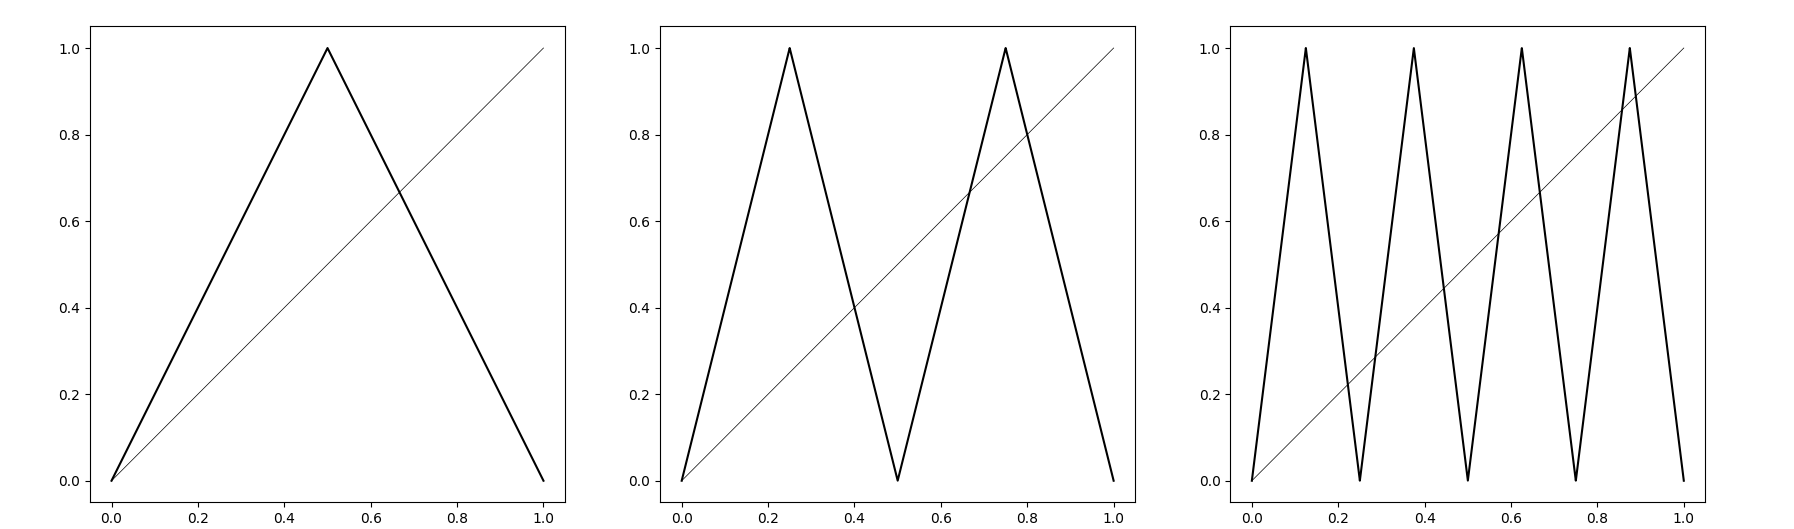
\includegraphics[scale=0.3]{images/tent-map.png}
\caption{Os gráficos de $T$, $T^2$ e $T^3$, respectivamente.}
\label{fig tent-map}
\end{figure}

\begin{theorem}
Se $\mu = 4$, então $h$ é caótica.
\end{theorem}

\begin{proof}
Basta observar que $\tau \circ T = h \circ \tau$, onde $\tau: [0, 1] \to [0, 1]$ é o homeomorfismo dado por $\tau(x) = \sen^2(\frac{\pi x}{2})$.
\end{proof}
